\documentclass[aps, pra, 10pt, twocolumn, superscriptaddress,floatfix]{revtex4-1}

\usepackage{amsmath,amssymb,amsfonts}
\usepackage{braket}
\usepackage[breaklinks=true,colorlinks,citecolor=blue,linkcolor=blue,urlcolor=blue]{hyperref}
\usepackage{mathtools}
\usepackage{dsfont}
\usepackage{algorithm}
\usepackage{algc}
\usepackage{algcompatible}
\usepackage{algpseudocode}
%
%
\newtheorem{thm}{Theorem}[section]

%%
\def \id {\mathds{1}}
\def \abs {\text{Abs}}
\newcommand{\norm}[1]{\lVert#1\rVert}
\DeclareMathOperator{\tr}{Tr}
\newcommand{\round}[1]{\ensuremath{\lfloor#1\rceil}}

\begin{document}
%
\title{Bayesian phase estimation with q-plates}

\begin{abstract}
	In this notes I will discuss some possible modifications of the resampling strategy in the particle filter algorithm for the task of phase estimation, in order to find the most suitable procedure. Still to implement are the estimation of the visibilities, a way to force the measurements with same quantum resource to be performed next to one another, and the possibility to perform arbitrary polarization measurements. In particular we want to address the concern that the tails of the posterior probability distribution, that are meaningful in the phase estimation problem could be depleted by the repeated resampling of the particles ensemble. We explore the possibility of using a procedure of importance resampling, but conclude that it isn't really needed, and the simple multinomial resampling seems to suffice. Importantly we also see that the resampling proposed in~\cite{Granade2012} doesn't seem to always work very well. Furthermore, the algorithm converges quickly to the true value of the phase also if we do not resample. \textbf{Important: the paper in~\cite{Wiebe2020} tries to solve exactly the problem that I wanted to attack with importance resampling.}
\end{abstract} 
%

\author{Federico Belliardo}
\email{federico.belliardo@sns.it}
\affiliation{NEST, Scuola Normale Superiore, I-56126 Pisa,~Italy}

\maketitle


\section{Particle filter for a phase estimation problem}
%
We might try to abandon our original phase estimation algorithm to pursue a joint Bayesian estimation of the phase and the visibilities, based on the approach presented in \cite{Granade2012}. The set of possible experimental controls is the size of the quantum resources to be used (the charge of the q-plates in our situation) together with the polarization that we choose to measure (indicated with $0$ and $\frac{\pi}{2}$), therefore $c_i \in \lbrace (1, 0), (1, \frac{\pi}{2}) , (s_2, 0), (s_2, \frac{\pi}{2}), \dots, (s_K, 0), (s_K, \frac{\pi}{2}) \rbrace$, with $c_i$ being the control used at the $i$-stage of the Bayesian procedure. At stage $N$ we will have used the controls $C = \lbrace c_1, c_2, c_3, \dots, c_N \rbrace$. The result of the experiment at stage $i$ is denoted with the letter $d_i$, and $D = \lbrace d_1, d_2, d_3 \cdots, d_N \rbrace$ indicates the sequence of results up to stage $N$. The core of the Bayesian procedure in \cite{Granade2012} is the maximization of a certain utility function $U \left( c_{N+1}, C\right)$ with respect to the next strategy selection $c_{N+1}$. The utility function is the circular variance of the posterior probability distribution after the measurement $c_{N+1}$ appropriately weighted for all the possible outcomes $d_{N+1}$. The algorithms to compute estimators of the circular mean and variance are reported in Algorithm~\ref{alg:meanVarEstimation}, and the utility function in Algorithm~\ref{alg:utilityNVcircular}. The function guessExperiment is implemented to trivially return a random experiment among the finite set of possible ones, while the localOptimization function scans the small number of possible experiments and exactly returns the optimal one.
%
\begin{algorithm}[H]
	\caption{Mean and variance estimation}
	\label{alg:meanVarEstimation}
	\begin{algorithmic}[1]
		\Function{estMeanCircular}{$\lbrace \theta_i \rbrace, \lbrace w_i \rbrace$}
		\State \Return $\hat{\mu} \gets  \arg \left[ \sum_i w_i \exp(i \theta_i) \right] \mod 2 \pi$
		\EndFunction
	\end{algorithmic}
	
	\begin{algorithmic}[1]
		\Function{estVarianceCircular}{$\lbrace \theta_i \rbrace, \lbrace w_i \rbrace$} 
		\State $z \gets \sum_i w_i \exp(i \theta_i)$ 
		\State $R \gets \norm{z}$
		\State \Return $\hat{\sigma} \gets \sqrt{-2 \log(R)}$
		\EndFunction
	\end{algorithmic}
\end{algorithm}
%
%
\begin{algorithm}[H]
	\caption{Circular utility function}
	\label{alg:utilityNVcircular}
	\begin{algorithmic}[1]
	\Function{utilityNVCircular}{$\lbrace \theta_i \rbrace , \lbrace w_i \rbrace, s, \phi$}	
		\For {$D \in \lbrace -1, +1 \rbrace$}
			\State $\lbrace w_i' \rbrace \gets \Call{weightsUpdate}{\lbrace \theta_i \rbrace , \lbrace w_i \rbrace, D, s, \phi}$
			\State $u_D \gets - \Call{estVarianceCircular}{\lbrace \theta_i \rbrace, \lbrace w_i' \rbrace}$
			\State $u_D \gets u_D \cdot \sum_{i} w_i \text{Pr} \left(D | \theta_i, s, \phi \right)$
		\EndFor
		\State \Return $\sum_{D} u_D$
	\EndFunction 
	\end{algorithmic}
\end{algorithm}
%
The conditional probability distribution $\text{Pr} \left(D | \theta, s, \phi \right)$ is
%
\begin{equation}
	\text{Pr} \left(D | \theta, s, \phi \right) = \frac{1 - D \cos (s \theta + \phi) }{2} \; ,
\end{equation}
%

\section{Resampling}
%
In the following we indicate with the apex the quantities after the resampling, for example $w_i$ are the weights pre-resampling and $w_i'$ are the weights post-resampling. The Bayesian update of~\cite{Granade2012} remains untouched, while for the resampling procedure we have several proposal. We start from the one presented in~\cite{Granade2012}, and adapt it to the estimation of a phase, that means the combination $a \theta_j + (1-a) \hat{\mu}$ should be interpreted as a combination on the unitary circle, and the angle $\tilde{\theta}_i$ extracted from a normal distribution should be cast in the interval $[0, 2 \pi]$.
%
\begin{algorithm}[H]
	\caption{Circular resampling}
	\label{alg:resamplingCircular}
	\begin{algorithmic}[1]
		\Function{resamplingCircular}{$\lbrace \theta_i \rbrace, \lbrace w_i \rbrace$, $n_{part}'$, $a$}
		\State $\hat{\mu} \gets \Call{estMeanCircular}{\lbrace \theta_i \rbrace, \lbrace w_i \rbrace}$
		\State $h \gets \sqrt{1-a^2}$
		\State $\hat{\sigma} \gets h^2 \Call{estVarianceCircular}{\lbrace \theta_i \rbrace, \lbrace w_i \rbrace}$
		\For {$i = 1 \to n_{part}'$}
		\State draw $j$ with probability $w_j$
		
		\If{$\theta_j - \hat{\mu} > \pi$}
		\State $\mu_i \gets a (\theta_j - 2 \pi) + (1-a) \hat{\mu} \mod 2 \pi$
		\ElsIf{$\hat{\mu} - \theta_j > \pi$}
		\State $\mu_i \gets a \theta_j + (1-a) (\hat{\mu} - 2 \pi) \mod 2 \pi$
		\Else 
		\State $\mu_i \gets a \theta_j + (1-a) \hat{\mu}$
		\EndIf		
		\State draw $\tilde{\theta}_i$ from $\mathcal{N} \left( \mu_i, \hat{\sigma} \right)$
		\State $\theta_i' \gets \tilde{\theta}_i \mod 2 \pi$
		\State $w_i' \gets 1/n_{part}'$
		\EndFor
		\EndFunction
	\end{algorithmic}
\end{algorithm}
%
We indicate with $n_{part}$ the number of particles in the old ensemble and with $n_{part}'$ the number in the new ensemble. In all the simulation of this note we set $n_{part}' = n_{part}$. The Algorithm~\ref{alg:resamplingCircular} assumes a unimodal posterior and draws new locations for the particles at each resampling. With respect to the algorithm presented in~\cite{Granade2012} we have adapted it to a circular variable. It is although not the simplest resampling procedure we can think of, which is Algorithm~\ref{alg:resamplingSimplified}. This procedure draws the new particles from a multinomial with outcomes $j \in \lbrace1, \dots, n_{part} \rbrace$ and assigns to the extracted particles a uniform distribution.
%
\begin{algorithm}[H]
	\caption{Simplified resampling}
	\label{alg:resamplingSimplified}
	\begin{algorithmic}[1]
		\Function{resamplingSimplified}{$\lbrace \theta_i \rbrace, \lbrace w_i \rbrace$, $n_{part}'$}
		\For {$i = 1 \to n_{part}'$}
		\State draw $j$ with probability $w_j$
		\State $\theta_i' \gets \theta_j$
		\State $w_i' \gets 1/n_{part}'$
		\EndFor
		\EndFunction
	\end{algorithmic}
\end{algorithm}
%
The resampling procedure converts weights in density of particles by sampling from the probability distribution
%
\begin{equation}
	p(\theta) = \sum_i w_i \delta(\theta-\theta_i) \; .
\end{equation}
%
That is, after resampling, in every interval $[\theta, \theta + \Delta \theta]$ we expect to find a number of particles 
%
\begin{equation}
	N'([\theta, \theta + \Delta \theta]) := \sum_i \chi_{[\theta, \theta + \Delta \theta]} (\theta_i') \; ,
\end{equation}
%
proportional to the total weight pre-resampling
%
\begin{equation}
	W([\theta, \theta + \Delta \theta]) := \sum_{i} w_i \chi_{[\theta, \theta + \Delta \theta]} (\theta_i) = \int_{\theta}^{\theta + \Delta \theta} p(\theta) d \theta \; ,
\end{equation}
%
Because the weights of the new resampled ensemble are uniformly initialized we are representing the same posterior probability distribution before and after the resampling. However we can think of a more general resampling procedure, called \textbf{importance resampling}. Now the particles are sampled from a custom probability distribution $\pi (\theta)$. That is, their density satisfies
%
\begin{equation}
	N'([\theta, \theta + \Delta \theta]) \propto \pi(\theta) \Delta \theta \; .
\end{equation}
%
We can adjust the weights in the new ensemble $\lbrace \theta_i', w_i' \rbrace$, in such a way that it represents again the posterior probability distribution, that means we want to impose
%
\begin{equation}
	W'([\theta, \theta + \Delta \theta]) \sim p(\theta) \Delta \theta \; .
\end{equation}
%
Let us consider the weights of the particles in $[\theta, \theta+\Delta \theta]$ to be constant across the interval ($w := w_i = \text{const.}$) and write
%
\begin{equation}
	W'([\theta, \theta + \Delta \theta]) = w N'([\theta, \theta + \Delta \theta]) \sim w \pi(\theta) \Delta \theta \; ,
\end{equation}
%
if we impose $w \pi(\theta) \Delta \theta \sim p(\theta) \Delta \theta$, we get $w_i = w \sim \frac{p(\theta)}{\pi (\theta)}$ for the particles in the interval $[\theta, \theta+\Delta \theta]$. The advantage of performing such contrived procedure is that we might enhance the tails of the posterior in $\pi(\theta)$ in order not to lose them during the resampling and then assign the particles the appropriate weights. We will therefore choose
%
\begin{equation}
	\pi (\theta) \sim f(\theta) p(\theta) \; ,
\end{equation}
%
where $f(\theta)$ is an appropriate function that enhances the tails of $p(\theta)$. In the appendix we comment on this choice but for the moment we take
%
\begin{equation}
	f(\theta) = 1 + \frac{1}{\hat{\sigma^2}} (\theta - \hat{\mu})^2 \; ,
\end{equation}
%
where $\hat{\sigma}$ and $\hat{\mu}$ are the estimated (circular) variance and mean of the particle ensemble and the distance $\theta - \hat{\mu}$ is the angular distance. The algorithm goes as following
%
\begin{algorithm}[H]
	\caption{Importance resampling}
	\label{alg:importanceResampling}
	\begin{algorithmic}[1]
		\Function{resamplingImportance}{$\lbrace \theta_i \rbrace, \lbrace w_i \rbrace$, $n_{part}'$}
		\State $\hat{\mu} \gets \Call{estMeanCircular}{\lbrace \theta_i \rbrace, \lbrace w_i \rbrace}$
		\State $\hat{\sigma} \gets \Call{estVarianceCircular}{\lbrace \theta_i \rbrace, \lbrace w_i \rbrace}$
		\For {$i = 1 \to n_{part}$}
		\State $w^\pi_i \gets w_i \cdot f(\theta_i)$
		\EndFor
		\State $w^\pi_i \gets w^\pi_i/\sum_{i} w^\pi_i$
		\For {$i = 1 \to n_{part}'$}
		\State draw $j$ with probability $w^\pi_j$
		\State $\theta_i' \gets \theta_j$
		\State $w_i' \gets w_j/w^\pi_j$
		\EndFor
		\State $w_i' \gets w_i'/\sum_{i} w_i'$
		\EndFunction
	\end{algorithmic}
\end{algorithm}
%
\subsection{Number of particles}
\label{sec:numPart}
%
In this subsection we argue that the minimum number of particles to be used is a small multiple of $\sqrt{N} \times \max{s}$. If the resampling algorithm is of the simplified type then the positions of the particles are generated at the beginning and are not changed during the execution (unless a noise is introduced). In the final stage of the estimation we get a central peak of size $\propto \frac{1}{\sqrt{N} \times \max{s}}$, or at least we don't expect it to be smaller than this values, therefore a number of points $k\sqrt{N} \times \max{s}$ is needed, where $k$ is the number of particles in the principal peak.
%
\begin{figure}[!t]
	\begin{center}
		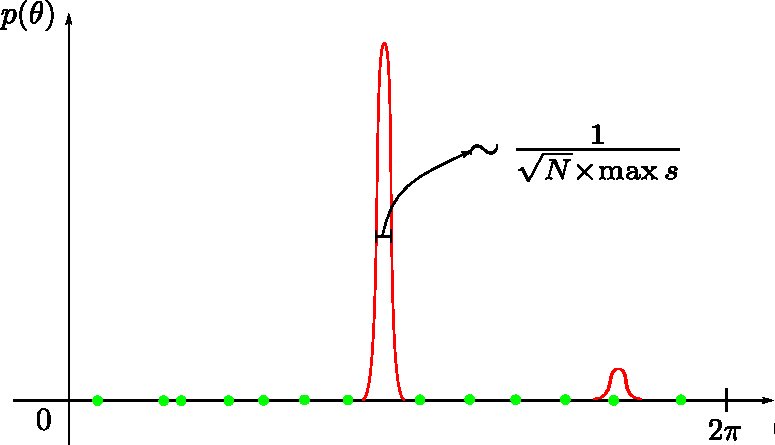
\includegraphics[width=0.45\textwidth]{immagini/numParticles.pdf}
	\end{center}
	\caption{In this example the selected points are too sparse and do not sample correctly the posterior probability distribution.}
	\label{fig:typicalPeak}
\end{figure}
%
Moreover the width of the other peaks in the distribution seems to be experimentally approximately the same of the central peak. In our simulation we took $k =10$. We also insert a lower bound to the number of particles, set arbitrarily to $n_{part} = 3000$. In summary 
%
\begin{equation}
	n_{part} = \max \lbrace \round{k \sqrt{N} \times \max{s}} , 3000 \rbrace \; .
\end{equation}
%
We stress that such analysis applies to the resampling algorithm that \textbf{do not} change the locations of the particles. Those that do, like the Circular resampling, might not be subject to it.


\subsection{Simulations results}
%
In this section we report the results of the simulations for the three resampling algorithms. All the simulations refer to the estimation of the single angle $\theta = 1 \, \text{rad}$, the number of experiments runs from $N = 10$ to $N = 200$ with step $10$. Each point is the the result of $\nu = 30$ simulation that gave estimations $\hat{\theta}_i$ with $i = 1, 2, \dots, \nu$ as results. We plot the MSE
%
\begin{equation}
	\Delta^2 \hat{\theta} = \frac{1}{\nu} \sum_{i=1}^\nu (\hat{\theta}_i - \theta)^2 \; .
\end{equation}
%
as a function of the number of experiments $N$, that is the number of photons used. The number of particles has been chosen according to the rule presented in section~\ref{sec:numPart}, in all cases the resampling threshold has been set to $0.5$. The circular version of the resampling seems to be particularly affected from the tails of the probability distribution. We see indeed that the estimation fails to reach the desired precision. The other strategies give comparable results. In particular there doesn't seems to be a difference between the strategy with the importance resampling and the strategy with the simplified resampling. \textbf{We conclude therefore that the importance resampling is not needed}.
%
\begin{figure}[!t]
	\begin{center}
		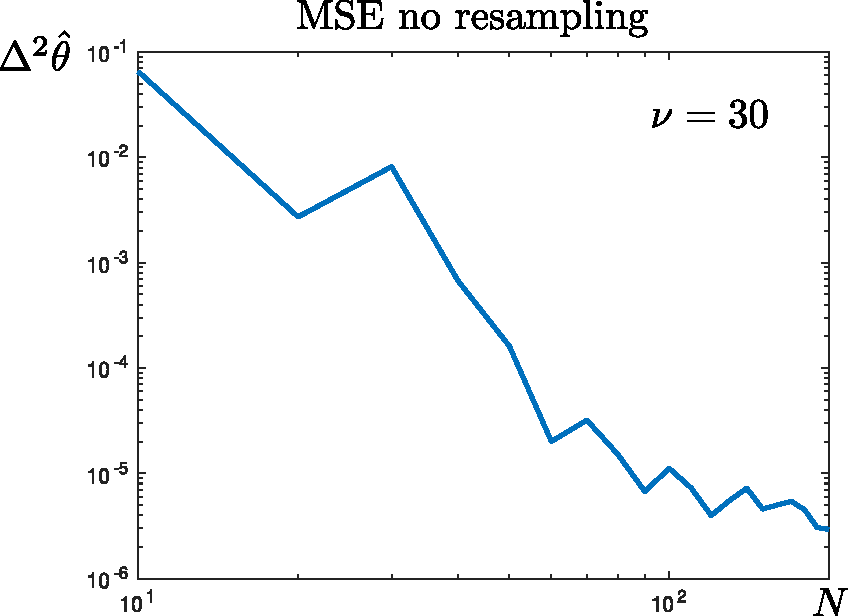
\includegraphics[width=0.45\textwidth]{immagini/noResampling.pdf}
	\end{center}
	\caption{MSE precision for an experiment with no resampling.}
	\label{fig:noResampling}
\end{figure}
%
\begin{figure}[!t]
	\begin{center}
		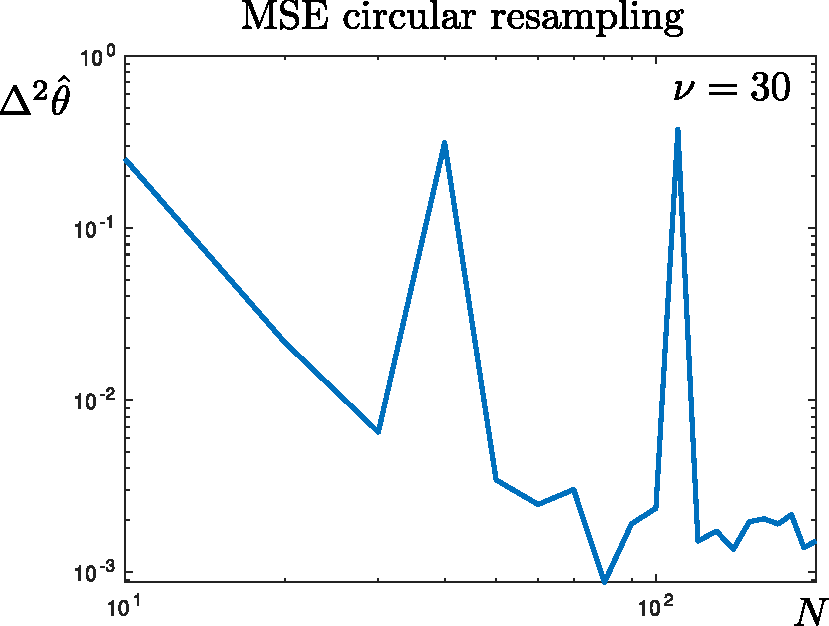
\includegraphics[width=0.45\textwidth]{immagini/circularResampling.pdf}
	\end{center}
	\caption{MSE precision for an experiment with circular resampling, and $a = 0.9$.}
	\label{fig:ircularResampling}
\end{figure}
%
\begin{figure}[!t]
	\begin{center}
		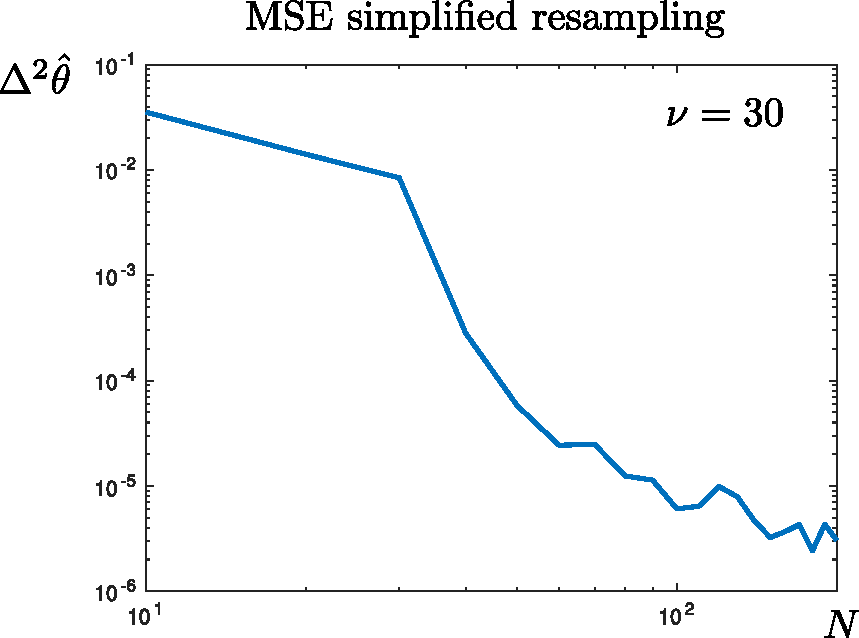
\includegraphics[width=0.45\textwidth]{immagini/simplifiedResampling.pdf}
	\end{center}
	\caption{MSE precision for an experiment with circular resampling, with $a = 0.9$.}
	\label{fig:simplifiedResampling}
\end{figure}
%
\begin{figure}[!t]
	\begin{center}
		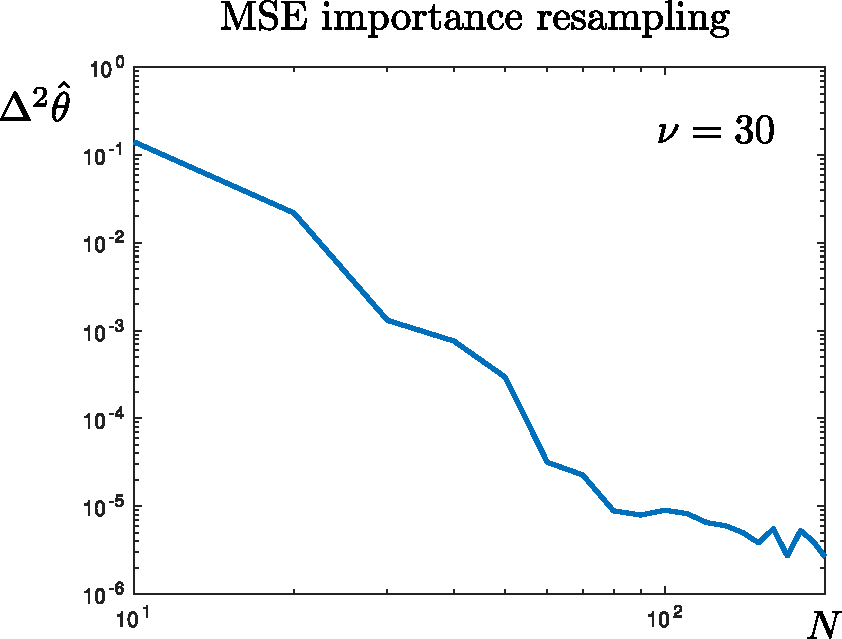
\includegraphics[width=0.45\textwidth]{immagini/importanceResampling.pdf}
	\end{center}
	\caption{MSE precision for an experiment with circular resampling, with $a = 0.9$.}
	\label{fig:importanceResampling}
\end{figure}
%

\section{Errata corrige original paper}
%
There seems to be some minor typos in the source paper~\cite{Granade2012}, that we proceed to list in this section
%
\begin{enumerate}
	
	\item p. 11, the computation of the variance $u_D \leftarrow - \sum_{i} w_i (\boldsymbol{x}_i - \boldsymbol{\mu})^T Q (\boldsymbol{x}_i - \boldsymbol{\mu})$ in Algorithm 5 should contain the updated weights $w_i'$. When estimating a phase this line should be $u_d \leftarrow - \text{estVarianceCircular} (\lbrace \theta_i, w_i' \rbrace)$, as in Algorithm~\ref{alg:utilityNVcircular}.
	
	\item p.12, in Algorithm 7 the resampling condition is $\frac{1}{\sum_{i} w_i^2} \le r \times n_{part}$.
	
\end{enumerate}

\section{Random perturbation}
%
After a resampling procedure with the simplified algorithm or with the importance sampling procedure the diversity of the ensemble is reduced. Because the same positions with high weights is replicated many times. After each resampling we add a Gaussian noise $\mathcal{N} (0, \sigma_p)$ to each particle in order to increase diversity, this procedure is called roughening. Doing so introduces a fundamental limit in the precision of the procedure $\sigma_p$, that should be chosen smaller than the maximum theoretical precision of the Bayesian learning, we chose therefore $\sigma_p = (\sqrt{N} \times \max s)^{-1}$. Some simulation have been performed introducing this noise, but \textbf{no measurable improvement has been observed.}

\appendix

\section{Form of the $f(\theta)$ function}
%
First of all let us indicate with $\theta_0$ the true value of the phase and with $\Delta \hat{\theta}$ the RMSE error $\Delta \hat{\theta} := \sqrt{\Delta^2 \hat{\theta}}$. A typical posterior probability distribution for the angle $\theta$ look like in Fig.~\ref{fig:typicalModified}. We have a central peak in the position of the true value $\theta_0$ and many scattered secondary peaks. Our objective is to find a function that enhances the secondary peaks and brings them to the level of the principal one.
%
\begin{figure}[!t]
	\begin{center}
		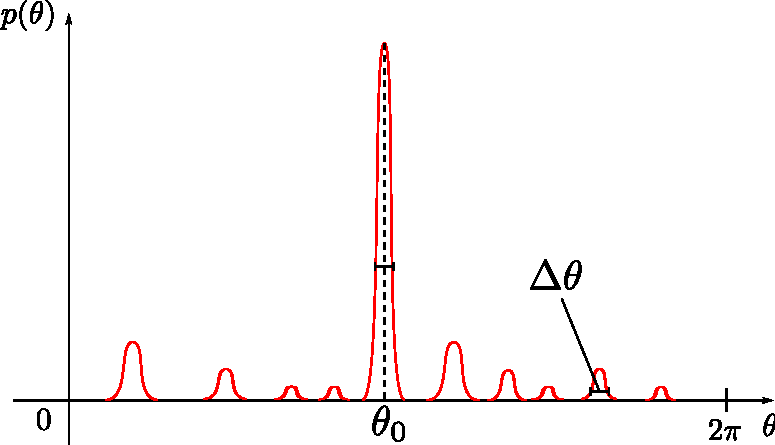
\includegraphics[width=0.45\textwidth]{immagini/typical.pdf}
	\end{center}
	\caption{Typical form of a posterior probability distribution. The secondary peaks are significantly lower that the principal one.}
	\label{fig:typicalModified}
\end{figure}
%
The form of the function $f(\theta)$ comes from an heuristic arguments that we discuss in this section. Experimentally we observe that the secondary peaks have size $\Delta \theta \simeq \Delta \hat{\theta}$, which is small for $N \gg 1$, so that we can consider the peak localized at its position $\theta$. Therefore its contribution to the MSE is
%
\begin{equation}
	\int p(\hat{\theta}) (\hat{\theta}-\theta_0)^2 d \hat{\theta} \sim \bar{p}(\theta) (\theta-\theta_0)^2 \Delta \hat{\theta} \; .
\end{equation}
% 
where $\bar{p}(\theta)$ is the characteristic probability of the peak. Such contribution must be relevant when compared to the MSE $\Delta^2 \hat{\theta}$:
%
\begin{equation}
	\bar{p}(\theta) (\theta-\theta_0)^2 \Delta \hat{\theta} \sim \Delta^2 \hat{\theta} \; ,
\end{equation}
%
that means those peaks with probability density 
%
\begin{equation}
	\bar{p}(\theta) \simeq \frac{\Delta \hat{\theta}}{(\theta-\theta_0)^2} \; .
\end{equation}
%
will contribute to the MSE. The function $f(\theta)$ is chosen to make the probability $\bar{p} (\theta) \Delta \hat{\theta}$ of sampling from the peak of order $\mathcal{O}(1)$, that is
%
\begin{equation}
	f(\theta) \hat{p} (\theta) \Delta \hat{\theta} \sim f(\theta) \frac{\Delta^2 \hat{\theta}}{(\theta-\theta_0)^2} \sim 1 \; . 
\end{equation}
%
Therefore on the secondary peaks the function $f(\theta)$ should have value $\sim \frac{(\theta-\theta_0)^2}{\Delta^2 \hat{\theta}}$, while near the principal one it should be $f(\theta) \sim 1$. We choose
%
\begin{equation}
f(\theta) = 1 + \frac{(\theta-\theta_0)^2}{\Delta^2 \hat{\theta}} \; ,
\end{equation}
%
as an interpolating approximation. Of course the true MSE and $\theta_0$ are unknown during the execution and we should use the approximate values $\hat{\mu}$ and $\hat{\sigma}$. Notice that the algorithm will perform a correct resampling for whatever reasonable function $f(\theta)$, it is a matter of choosing a convenient one. 



\begin{thebibliography}{100}
	
\bibitem{Granade2012} C E Granade et al 2012 \href{https://doi.org/10.1088/1367-2630/14/10/103013}{New J. Phys. {\bf 14} 103013}.

\bibitem{Wiebe2020} T. Ramakrishna and N. Wiebe, \href{http://arxiv.org/abs/2009.07898}{http://arxiv.org/abs/2009.07898}.

\bibitem{Hol2006} J D Hol, T B Schon, and F Gustafsson 2006 \href{http://ieeexplore.ieee.org/document/4378824/}{2006 IEEE Nonlinear Statistical Signal Processing Workshop}.

\bibitem{Li2015} T Li, M Bolic, and P M Djuric 2015 \href{https://ieeexplore.ieee.org/document/7079001/}{IEEE Signal Process. Mag. {\bf 32} 70-86}.


\end{thebibliography}

\end{document}